\documentclass[12pt,fleqn]{article}\usepackage{../../common}
\begin{document}
Materyel Mekaniği - 6

Direk Direngenlik Metotu (Direct Stiffness Method)

Direngenlik metotunu anlamak icin direngenlik matrisi kavramini islemek
gerekir. Bu konuya biraz [2]'de degindik. Bir oge grubunun, sistemin direngenlik
matrisi dugumsel yer degisimler $d$ ile dugumsel kuvvetler $F$'yi ilintilendiren
bir $K$ matrisidir, oyle ki [1, sf. 34]

$$
F = K d
$$

esitligi gecerlidir. Alttaki gibi bir sistem olsun,

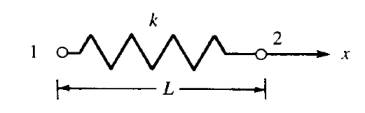
\includegraphics[width=15em]{phy_020_strs_06_03.jpg}

Sistemde bir yay goruluyor, bu yay uzerinde iki tane dugum noktasi sectik,
onlari takip edecegiz, dugum 1 ve 2. Dugumlerdeki yer degisimler $u_1,u_2$
olsun, yaydaki toplam degisimo $\delta = u_1 - u_2$. Uygulanan kuvvet $T$
ise bir sabit $k$ uzerinden $T = k \delta$ esitligi ortaya atilabilir.

Direngenlik matrisine gelirsek, sistemdeki tum yer degisimleri soyle gosterebiliriz,

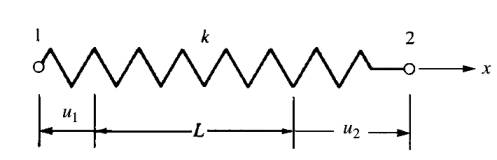
\includegraphics[width=15em]{phy_020_strs_06_04.jpg}

Sag ucta yay $T$ kuvveti ile cekiliyorsa, bu durum sol ucta $-T$ tepkisel
kuvvete sebep olur. Ayrica $u_1$'in sol yonu isaret ettigine dikkat, cunku yer
degisimin yonu pozitif yonun tersinde, yaydaki takip edilen nokta baslangic
aninin sol tarafinda kaliyor, bu sebeple yon eksi.

$$
f_{1x} = -T, \quad f_{2x} = T
$$

Hepsini bir araya koyarsak

$$
T = -f_{1x} = k (u_2 - u_1)
$$

$$
T = f_{2x} = k (u_2 - u_1)
$$

Yani

$$
f_{1x} = k(u_1 - u_2)
$$

$$
f_{2x} = k(u_2 - u_1)
$$

Matris formunu kullanrak usttekini soyle gosterebiliriz,

$$
\left[\begin{array}{ccc}
f_{1x} \\ f_{2x}
\end{array}\right] = 
\left[\begin{array}{ccc}
k & -k \\ -k & k
\end{array}\right]
\left[\begin{array}{ccc}
u_1 \\ u_2
\end{array}\right]
$$

Ifadenin ortasindaki 2 x 2 matrisi direngenlik matrisidir.

Ustdüşüm (Superposition)

Eger iki tane yay sistemini birbiriyle bagli olarak islemek istersek [1, sf. 38],
ustdusum teknigi kullanilabilir.

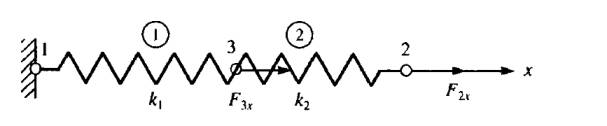
\includegraphics[width=20em]{phy_020_strs_06_02.jpg}

Iki yay var, birbirlerine baglilar, iki yayin sabitleri $k_1$, $k_2$
olsun. Her iki yayin direngenlik matrisi ayri ayri (tekabul eden yer degisim
degiskenleri matris kolon etiketi olarak gosteriliyor),

$$
k^{(1)} =
\begin{array}{cc} & \begin{array}{cc} u_1 & u_3 \end{array} \\ &
\left[
\begin{array}{cc}
k_1 & -k_1 \\ -k_1 & k_1
\end{array}
\right]
\end{array} 
\qquad
k^{(2)} =
\begin{array}{cc} & \begin{array}{cc} u_3 & u_2 \end{array} \\ &
\left[
\begin{array}{cc}
k_2 & -k_2 \\ -k_2 & k_2
\end{array}
\right]
\end{array}
$$





[devam edecek]


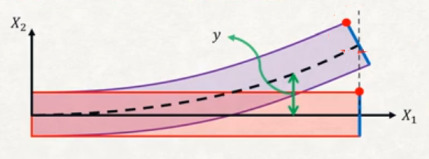
\includegraphics[width=20em]{phy_020_strs_06_01.jpg}


Kaynaklar

[1] Logan, {\em A First Course in the Finite Element Method}

[2] Bayramlı, {\em Hesapsal Bilim, Ders 1-8}

\end{document}
